\documentclass[aspectratio=169]{beamer}

\usepackage[utf8]{inputenc}
\usepackage{amsmath}
\usepackage{amsfonts}
\usepackage{amssymb}
\usepackage{graphicx}
\usepackage{ragged2e}
\usepackage{booktabs}
\usepackage{tabularx}
\usepackage{tikz}
\usetikzlibrary{calc, shapes, backgrounds}
\usepackage{amsmath}
\usepackage{amssymb}
\usepackage{dsfont}
\usepackage{url}
\usepackage{listings}
\usepackage[T1]{fontenc}

\usepackage{theme/beamerthemehbrs}

\author[Memon et al.]{%
  M.\,I.\ Memon \and U.\ Patil \and I.\ Awaad \and Y.\,M.\ Youssef}
\title{Learning Interpretable Scheduling Policies\\for Online Multi-Robot Task Allocation}
\subtitle{via Inductive Logic Programming -- PlanRob @ ICAPS 2026}
\institute[H-BRS]{Hochschule Bonn-Rhein-Sieg}
\date{ICAPS 2026, Dublin}
\subject{Multi-Robot Task Allocation}

\def\advisors{}
% \thirdpartylogo{path/to/logo}

\begin{document}

{
\begin{frame}
\titlepage
\end{frame}
}

% ============================================================
% MOTIVATION
% ============================================================
\begin{frame}{Motivation}
  \framesubtitle{Online task allocation in a dynamic warehouse}
  \begin{itemize}
    \item Fleet of mobile robots must fulfil a continuous stream of incoming orders
    \item Runtime decision: \alert{which robot handles which order?}
    \item Must account for battery level, proximity to shelf, and current workload
    \item NP-hard online scheduling -- practical systems rely on heuristic or learned policies
  \end{itemize}
  \vspace{0.4em}
  \begin{columns}[onlytextwidth]
    \column{.5\textwidth}
      \begin{exampleblock}{Existing approaches}
        Heuristics, auctions -- assign a robot and output a score or bid
      \end{exampleblock}
    \column{.47\textwidth}
      \begin{alertblock}{What they cannot do}
        Explain \emph{why} that robot was the right choice. No audit trail.
      \end{alertblock}
  \end{columns}
\end{frame}

% ============================================================
% PROBLEM FORMULATION
% ============================================================
\begin{frame}{Problem Formulation}
  \framesubtitle{$P_m \mid r_j,\, \mathrm{eligible} \mid C_{\max}$}
  \begin{columns}[onlytextwidth]
    \column{.52\textwidth}
      \begin{itemize}
        \item $m$ homogeneous robots as parallel machines
        \item Orders arrive online with release times $r_j$ -- no look-ahead
        \item Robot \textbf{eligible} iff idle and $b_r > b_{\min}$ (threshold 20\%)
        \item Processing time: $p_j = 2\,d(\text{drop-off},\, \text{shelf}_j)\,/\,v$
        \item Objective: minimise makespan $C_{\max}$
      \end{itemize}
    \column{.45\textwidth}
      \begin{block}{Why learn instead of derive?}
        \begin{itemize}
          \item NP-hard even offline ($m \geq 2$)
          \item Online LPT does not model eligibility
          \item \alert{Induce a policy from execution traces}
        \end{itemize}
      \end{block}
      \begin{alertblock}{Deferral}
        No eligible robot $\Rightarrow$ order queued, not force-assigned
      \end{alertblock}
  \end{columns}
\end{frame}

% ============================================================
% SYSTEM ARCHITECTURE
% ============================================================
\begin{frame}{System Architecture}
  \framesubtitle{Three core ROS\,2 nodes + offline learning pipeline}
  \begin{columns}[onlytextwidth]
    \column{.35\textwidth}
      \small
      \begin{itemize}
        \item \textbf{Task Manager} -- receives orders, queries state, invokes strategy
        \item \textbf{Fleet Manager} -- tracks location/battery/availability; Nav2 dispatch
        \item \textbf{Shared Memory} -- shelf locations, drop-off pose
      \end{itemize}
      \vspace{0.3em}
      \begin{block}{\small Offline pipeline}
        \footnotesize Logs $\to$ Popper ILP $\to$ \texttt{learned\_rules.pl} $\to$ Janus bridge $\to$ runtime
      \end{block}
    \column{.62\textwidth}
      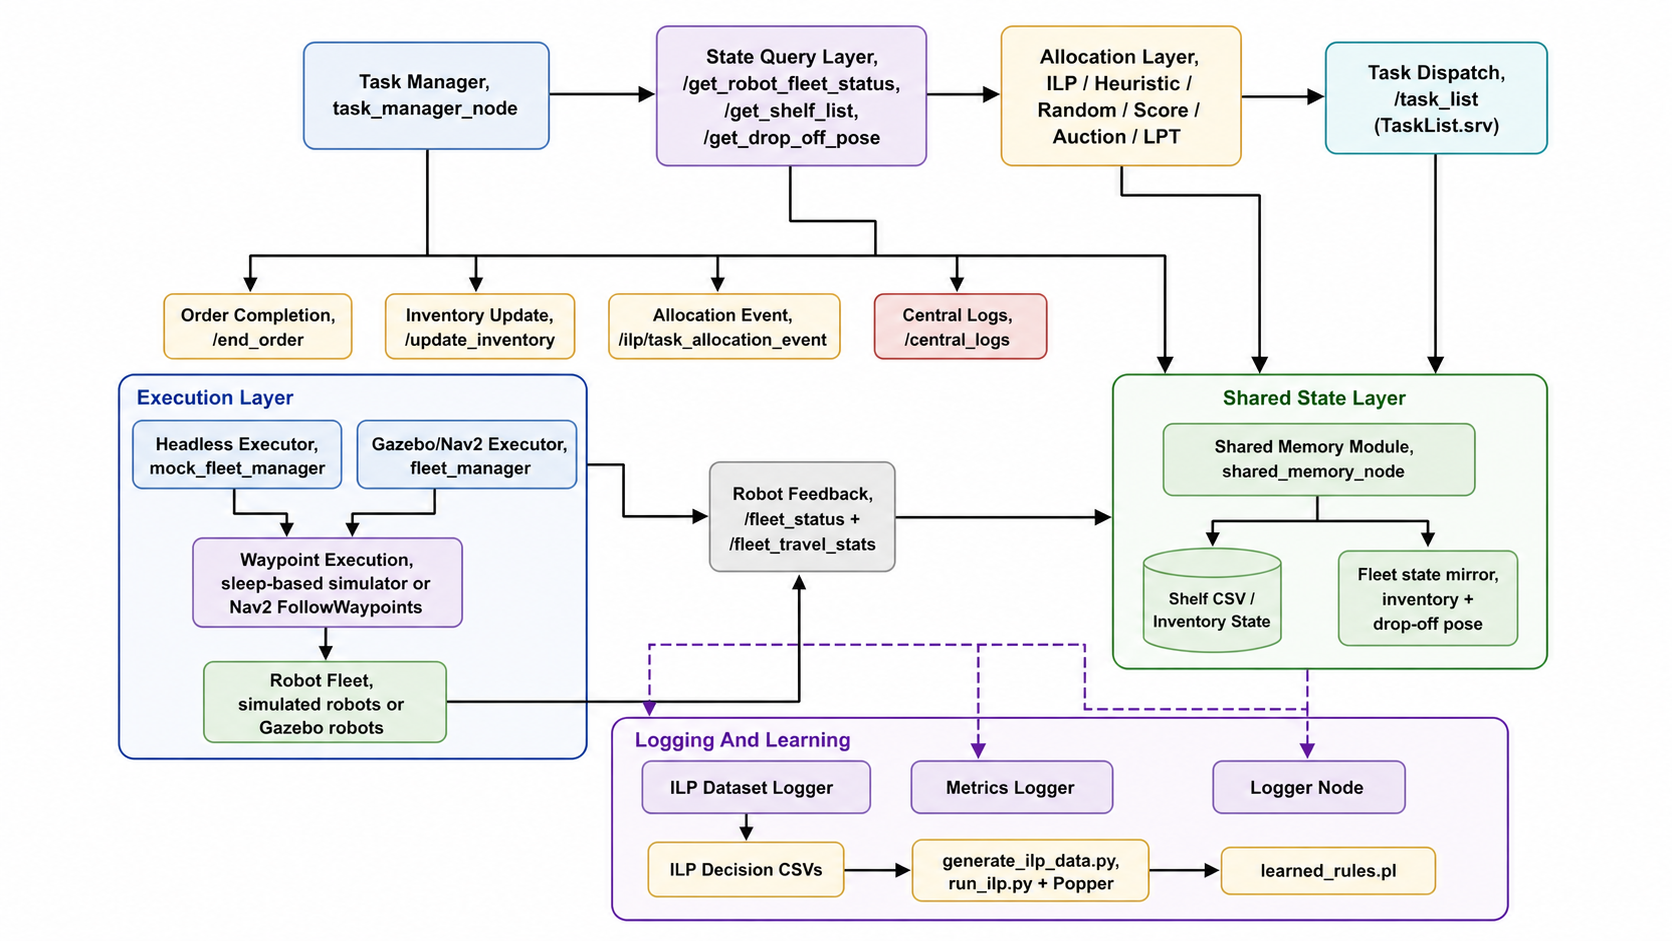
\includegraphics[width=\columnwidth]{figures/fig1_architecture.png}
  \end{columns}
\end{frame}

% ============================================================
% ILP LEARNING PIPELINE
% ============================================================
\begin{frame}[shrink=5]{ILP Learning Pipeline}
  \framesubtitle{From execution logs to symbolic Prolog rules}
  \begin{columns}[onlytextwidth]
    \column{.5\textwidth}
      \small
      \textbf{Training data:} one row per robot per allocation event\\
      (idle status, workload, battery, distance, dispatch decision)
      \vspace{0.3em}
      \textbf{Symbolic discretisation:}
      \begin{itemize}
        \item Battery $\to$ \texttt{\{low, medium, high\}}
        \item Distance $\to$ \texttt{\{near, medium, far\}}
        \item Workload $\to$ \texttt{\{zero, low, medium, high\}}
      \end{itemize}
      \vspace{0.3em}
      \textbf{Teacher (= Heuristic baseline):} eligibility $\to$ min workload $\to$ min distance
    \column{.47\textwidth}
      \begin{block}{Key derived predicates}
        \small
        \texttt{suitable\_robot(T,R)}\\
        \quad idle $+$ battery $> b_{\min}$\\[4pt]
        \texttt{closest\_least\_busy\_suitable(T,R)}\\[4pt]
        \texttt{no\_suitable\_robot(T)}
      \end{block}
      \vspace{0.3em}
      \begin{block}{Popper search}
        \small
        Targets: \texttt{assigned/2} and \texttt{defer/1}\\
        Max 3 rules, 4 variables, 5 literals
      \end{block}
  \end{columns}
\end{frame}

% ============================================================
% THE LEARNED POLICY
% ============================================================
\begin{frame}[shrink=5]{The Learned Policy}
  \framesubtitle{Two Prolog clauses induced by Popper from labelled allocation examples}
  \begin{columns}[onlytextwidth]
    \column{.5\textwidth}
      \begin{block}{}
        {\small\ttfamily
          assigned(T, R) :-\\
          \hspace{1.5em}closest\_least\_busy\_suitable(T, R).\\[0.4em]
          defer(T) :-\\
          \hspace{1.5em}no\_suitable\_robot(T).
        }
      \end{block}
      \vspace{0.3em}
      \begin{block}{Rule 1 in one sentence}
        Assign to the closest eligible idle robot with the lowest active workload
      \end{block}
    \column{.47\textwidth}
      \begin{exampleblock}{Scheduling interpretation}
        Three concepts in strict priority order:
        \begin{enumerate}
          \item Eligibility -- idle $+$ $b_r > b_{\min}$
          \item Load balance -- min workload tier
          \item Proximity -- min distance within tier
        \end{enumerate}
      \end{exampleblock}
      \begin{alertblock}{Rule 2}
        Deferral induced from data -- a learned precondition on action executability
      \end{alertblock}
  \end{columns}
\end{frame}

% ============================================================
% EXPLANATION GENERATION
% ============================================================
\begin{frame}[shrink=15]{Explanation Generation}
  \framesubtitle{Human-readable justification for every dispatch decision}
  \footnotesize
  \begin{table}
    \begin{tabularx}{\textwidth}{lXX}
      \textbf{Decision} & \textbf{Fleet State} & \textbf{Explanation} \\
      \toprule
      Assign &
        15 idle robots, all 100\%. R2 closest at 4.21\,m. &
        R2 matched \texttt{closest\_least\_busy\_suitable}.
        Cited: high battery, near, zero workload. \\
      \midrule
      Assign + tie-break &
        R10 and R14 tied at 4.70\,m. &
        Battery tie-break: R10 (100\%) over R14 (92.9\%).
        Tie-break reported explicitly. \\
      \midrule
      Defer &
        All 10 robots busy (workload 1). &
        All-busy is one instance where \texttt{no\_suitable\_robot(T)} holds.
        Learned rule \texttt{defer(T) :- no\_suitable\_robot(T)} fires. Task queued. \\
      \bottomrule
    \end{tabularx}
  \end{table}
  \vspace{0.2em}
  \begin{columns}[onlytextwidth]
    \column{.5\textwidth}
      \begin{block}{600 decisions}
        589 cited Rule 1 directly; 11 applied tie-break; 0 used fallback
      \end{block}
    \column{.47\textwidth}
      \begin{block}{Allocator runtime}
        5.75\,ms ($n=5$) -- 33.27\,ms ($n=15$); negligible vs.\ job execution time
      \end{block}
  \end{columns}
\end{frame}

% ============================================================
% EXPERIMENTAL SETUP
% ============================================================
\begin{frame}{Experimental Setup}
  \framesubtitle{Headless warehouse simulation -- reproducible without Gazebo}
  \begin{columns}[onlytextwidth]
    \column{.52\textwidth}
      \begin{itemize}
        \item 6 strategies: Random, Score, Heuristic, Auction, Online LPT, \alert{ILP}
        \item 4 fleet sizes: $n \in \{5, 10, 15, 20\}$ -- resource-constrained to over-provisioned
        \item 50 orders at 1\,Hz per trial; 3 trials; seeded RNG
        \item $v=2.0$\,m/s, drain 0.7\%/m, recharge 5\%/s, $b_{\min}=20\%$
        \item All 6 strategies: \textbf{100\% task success rate}
      \end{itemize}
    \column{.45\textwidth}
      \begin{block}{Regimes}
        \small
        $n=5$\quad resource-constrained (hardest)\\[3pt]
        $n=10$\quad moderately provisioned\\[3pt]
        $n=15$\quad lightly loaded\\[3pt]
        $n=20$\quad over-provisioned
      \end{block}
  \end{columns}
\end{frame}

% ============================================================
% RESULTS: MAKESPAN
% ============================================================
\begin{frame}[shrink=5]{Results: Makespan}
  \framesubtitle{Mean makespan (s) -- lower is better; bold = best per fleet size}
  \begin{columns}[onlytextwidth]
    \column{.44\textwidth}
      \small
      \begin{table}
        \begin{tabularx}{\columnwidth}{lrrrr}
          \textbf{Strategy} & \textbf{n=5} & \textbf{n=10} & \textbf{n=15} & \textbf{n=20} \\
          \toprule
          Random     & 162.1 & 83.0  & \textbf{62.9} & 63.0 \\
          Score      & 161.8 & 79.7  & 63.6          & 64.0 \\
          Heuristic  & 159.8 & 78.5  & 64.1          & \textbf{61.9} \\
          Auction    & 160.9 & 78.2  & 63.6          & 62.0 \\
          \alert{ILP}& \alert{\textbf{159.4}} & \alert{\textbf{77.6}} & 63.8 & 61.9 \\
          Onl.\ LPT  & 161.9 & 79.2  & 63.9          & 66.0 \\
          \bottomrule
        \end{tabularx}
      \end{table}
      \vspace{0.2em}
      \small ILP average rank: \alert{\textbf{2.0}} across all fleet sizes\\
      (Auction 2.75 $\cdot$ Heuristic 3.0 $\cdot$ Online LPT 5.0)
    \column{.53\textwidth}
      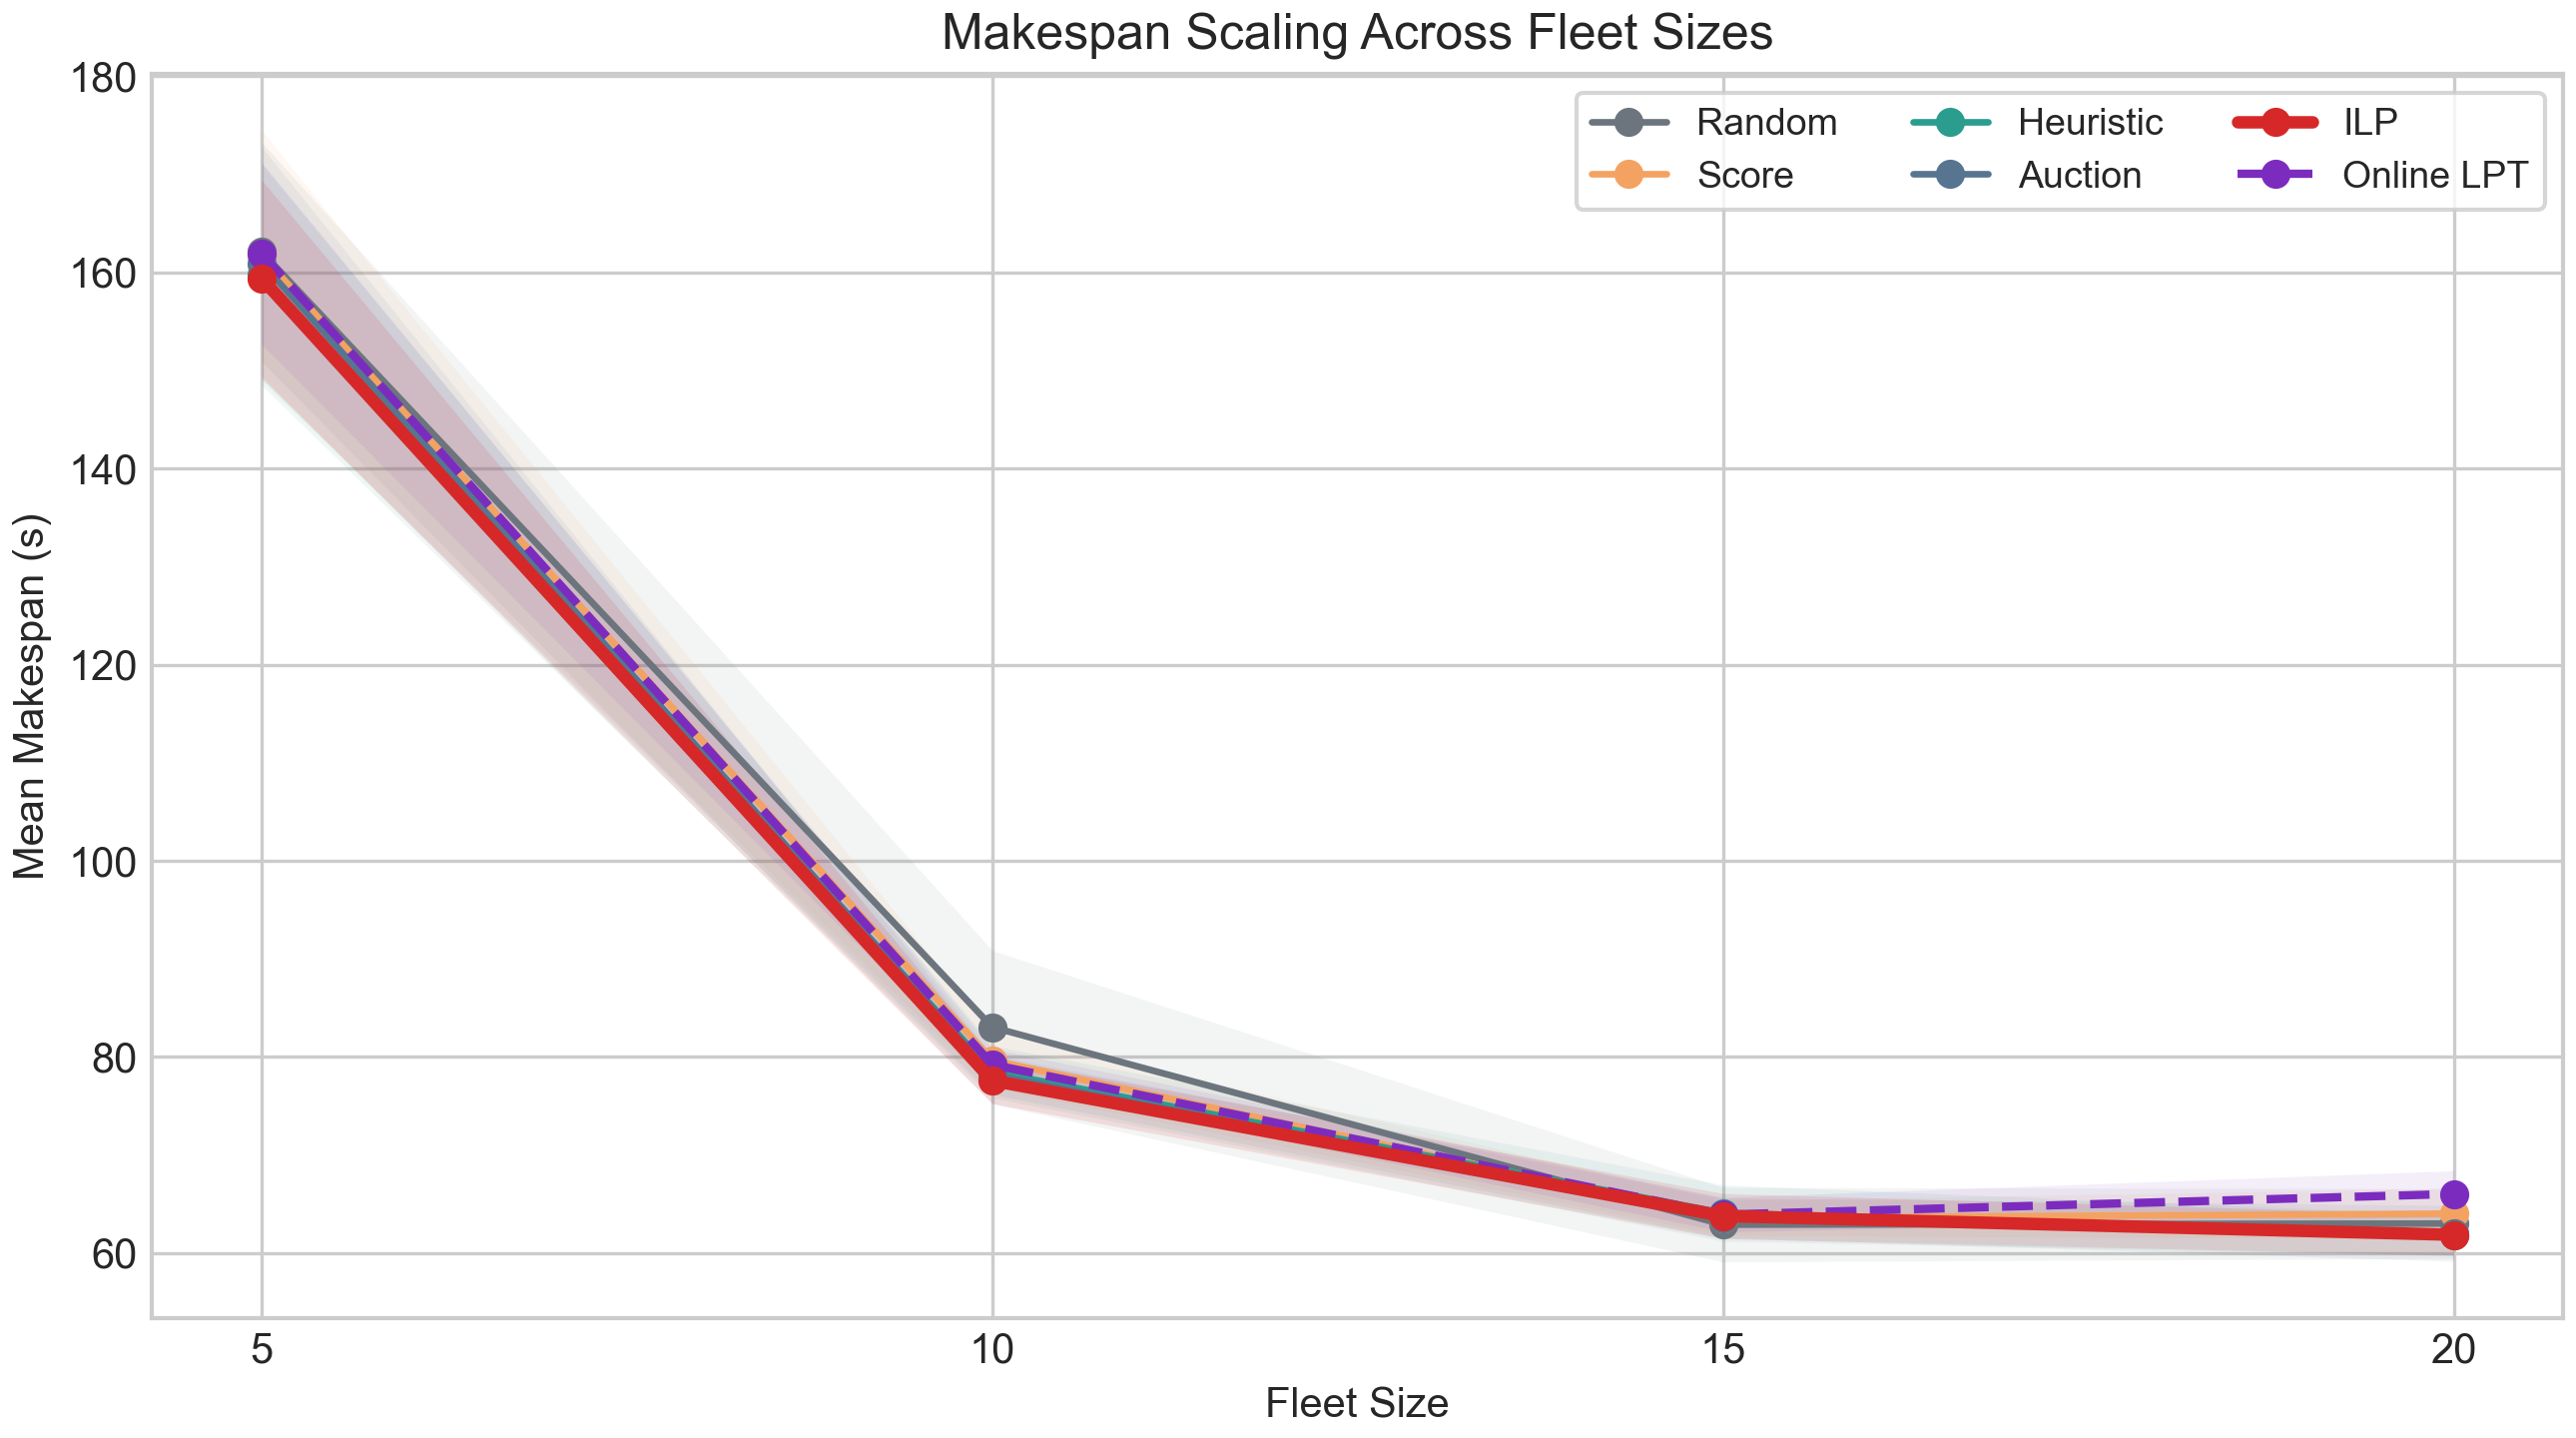
\includegraphics[width=\columnwidth]{figures/fig2_makespan.png}
  \end{columns}
\end{frame}

% ============================================================
% RESULTS: OVERALL RANKING
% ============================================================
\begin{frame}{Results: Overall Ranking}
  \framesubtitle{Ranking heatmap -- darker = better rank (1 = best)}
  \begin{columns}
    \column{.45\textwidth}
      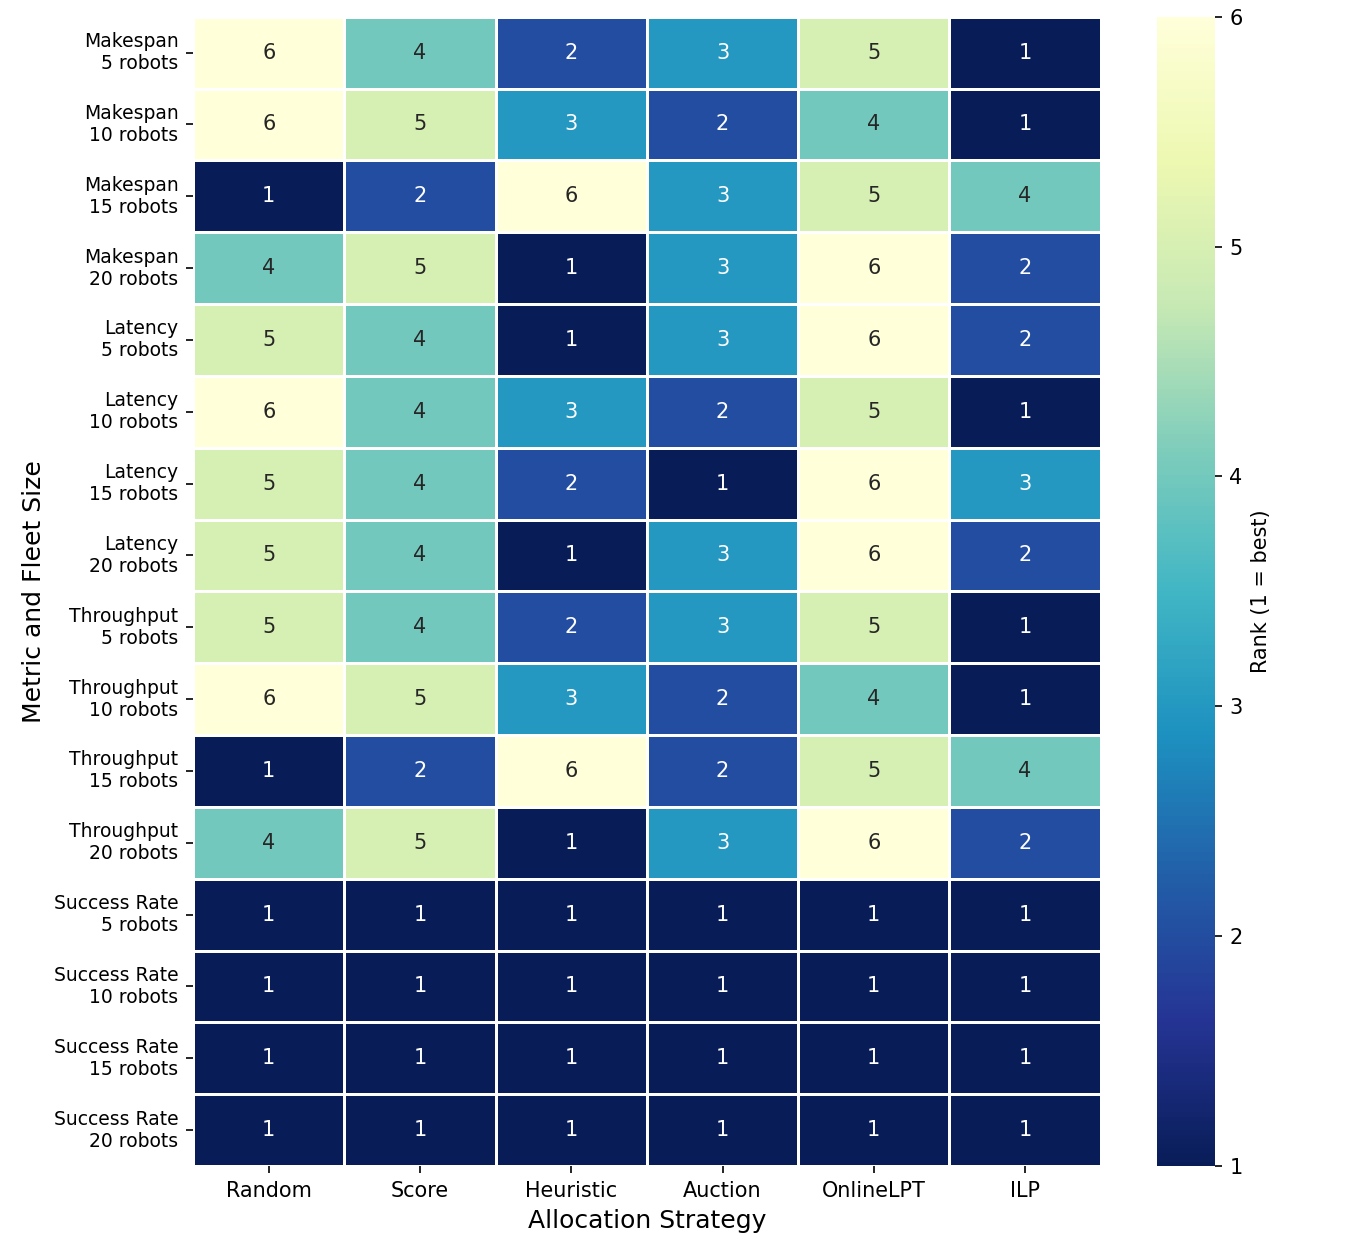
\includegraphics[width=\columnwidth]{figures/fig3_ranking.png}
    \column{.6\textwidth}
      \begin{block}{Key findings}
        \begin{itemize}
          \item ILP is empirically competitive; strongest at $n=5$, $n=10$ where deferral matters most
          \item At $n=20$: all top strategies within 0.17\,s -- margins are small
          \item Heuristic is the teacher: ILP's contribution is compressing that behavior into 2 executable symbolic rules
          \item \alert{Uniquely: a human-readable justification for every decision -- no baseline provides this}
        \end{itemize}
      \end{block}
  \end{columns}
\end{frame}

% ============================================================
% CONCLUSION
% ============================================================
\begin{frame}[shrink=5]{Conclusion}
  \begin{enumerate}
    \item \textbf{ILP learns the scheduling rule without being given the objective function or algorithm}\\
      \small Popper received only labelled traces over a scheduling-relevant predicate vocabulary.
      It recovered the allocation rule and deferral condition from data alone.
    \normalsize
    \vspace{0.3em}
    \item \textbf{Empirically competitive -- best average rank (2.0) over 3 trials per fleet size}\\
      \small Strongest under congestion; resource usage (travel, battery) matches the best hand-coded baselines at all fleet sizes.
    \normalsize
    \vspace{0.3em}
    \item \textbf{Human-readable audit trail -- absent from all evaluated baselines}\\
      \small Every dispatch decision justified by matched rule conditions; no post-hoc interpretation required.
  \end{enumerate}
  \vspace{0.3em}
  \begin{block}{Future work}
    \small Heterogeneous fleets $\;\cdot\;$ Stochastic arrivals $\;\cdot\;$ Online retraining $\;\cdot\;$ Larger fleet scaling
  \end{block}
\end{frame}

% ============================================================
% BACKUP A: Limitations
% ============================================================
\begin{frame}[shrink=10]{Limitations}
  \framesubtitle{Backup -- for Q\&A}
  \begin{itemize}
    \item Only 3 trials per fleet size -- trends are consistent but no confidence intervals reported
    \item Homogeneous fleet -- all robots identical speed, payload, battery dynamics
    \item Fixed 1\,Hz arrival rate -- Poisson arrivals not evaluated (deferral rule is stateless, generalization expected)
    \item Allocator runtime grows with fleet size: 33\,ms at $n=15$; Prolog assert/retract may need optimization at scale
    \item Online retraining pipeline implemented but not evaluated
    \item Atomic orders only -- task decomposition assumed upstream
  \end{itemize}
\end{frame}

% ============================================================
% BACKUP B: Secondary Metrics
% ============================================================
\begin{frame}{Secondary Metrics}
  \framesubtitle{Backup -- for Q\&A}
  \small
  \begin{table}
    \begin{tabularx}{\textwidth}{Xrrr}
      \textbf{Strategy} & \textbf{Runtime (ms)} & \textbf{Travel (m)} & \textbf{Battery (\%)} \\
      \toprule
      Random      &  0.097 & 23.85 & 16.70 \\
      Score       &  0.101 & 22.53 & 15.77 \\
      Heuristic   &  0.095 & 21.96 & 15.37 \\
      Auction     &  0.098 & 22.02 & 15.41 \\
      \alert{ILP} & \alert{16.257} & \alert{21.98} & \alert{15.38} \\
      Online LPT  &  0.087 & 24.02 & 16.81 \\
      \bottomrule
    \end{tabularx}
    \caption{ILP travel and battery match Heuristic/Auction. Runtime is ${\sim}160\times$ higher but negligible vs.\ job execution time (seconds).}
  \end{table}
  \vspace{0.2em}
  \small ILP deferral rate: 58.2\% at $n=5$ $\to$ 31.8\% at $n=10$ $\to$ 0.7\% at $n=15$ $\to$ 0\% at $n=20$
\end{frame}

\end{document}
